%%%%%%%%%%%%%%%%%%%%%%%%%%%%%%%%%%%%%%%%%%%%%%%

% Start with going to Settings/packages.tex and change the pdftitle and pdfauthor variables.

% Then make changes to pages in the Content folder, such as abstract, acknowledgement, declaration, supervisor and titlepage.

% Add your citations in the BibTex format in the citation.bib file. These can be found via the publisher website.

% Finally, add your content to chapters and appendices. Read all of them first as there might be some command explained there that you don't know. Additionally, add your figures to the Figure folder to keep them organised.

% Keep adding new chapters and appendices at their relevant places.

%%%%%%%%%%%%%%%%%%%%%%%%%%%%%%%%%%%%%%%%%%%%%%%

%% document class
\documentclass[12pt, a4paper, twoside]{article}

\usepackage{subfiles}
%% packages
%------------------------------------------------------------------------------------
%	PACKAGES AND OTHER DOCUMENT CONFIGURATIONS
%-------------------------------------------------------------------------------------

\usepackage{xcolor} % Required for specifying custom colours
\definecolor{grey}{rgb}{0.9,0.9,0.9} % Colour of the box surrounding the title

\usepackage[utf8]{inputenc} % Required for inputting international characters
\usepackage[T1]{fontenc} % Output font encoding for international characters
\usepackage{graphicx} % used for \includegraphics
\usepackage{float}
\usepackage{booktabs}
\usepackage{pdfpages}
\usepackage{subcaption}
\usepackage{tikz}
\usepackage{blindtext} % used for dummy texts
\usepackage{amsmath} % used for \eqref to refer to any labeled math equation
\usepackage{amssymb} % used for mathematical symbols
\usepackage{lettrine}

%% \usepackage{makeidx}
%% \makeindex

%\usepackage[ backend=biber, citestyle=authoryear-comp, sorting=ynt]{biblatex}
\usepackage[sort]{natbib}
\bibliographystyle{abbrvnat}
\setcitestyle{authoryear,open={(},close={)}} %Citation-related commands

\usepackage{epigraph}

\usepackage{titlesec, blindtext, color}
\definecolor{gray75}{gray}{0.75}
\newcommand{\hsp}{\hspace{20pt}}
\titleformat{\chapter}[hang]{\Huge\bfseries}{\thechapter\hsp\textcolor{gray75}{|}\hsp}{0pt}{\Huge\bfseries}[\headrule]

\usepackage[colorlinks=True, breaklinks]{hyperref} % to add links
%% \usepackage[hyphenbreaks]{breakurl} % break long urls
\renewcommand{\figureautorefname}{Fig}
\renewcommand{\equationautorefname}{Eq}

\definecolor{c1}{rgb}{0,0.3,0.9}
\hypersetup{
    linkcolor={c1},
    citecolor={c1},
    urlcolor={c1},
    pdftitle  = {BTP - 180106007},
    pdfauthor = {Aditi Madkaikar}
}

\usepackage[toc,page]{appendix}
\usepackage{subfig}
\usepackage{multirow}
\usepackage{array}

\usepackage{longtable}
%%\renewcommand{\baselinestretch}{}

\renewcommand{\labelenumi}{\arabic{enumi}.}
\usepackage{setspace}

\newcommand{\HRule}{\rule{\linewidth}{0.5mm}} % Defines a new command for the horizontal lines, change thickness here

\newcommand{\quickwordcount}[1]{%
    \immediate\write18{texcount -1 -sum -merge #1.tex > #1-words}%
    \input{#1-words}words%
}

\usepackage{parskip}

\usepackage{datetime}
\newdateformat{monthyeardate}{\monthname[\THEMONTH] \THEYEAR}
%\addbibresource{Content/citation.bib}
\usetikzlibrary{positioning}
\graphicspath{{../results/}}
%% page settings
%-------------------------------------------------------------------------------------
%	PAGE SETTINGS
%-------------------------------------------------------------------------------------

\usepackage[right=2cm, left=2cm, top=2.5cm, bottom=2cm]{geometry}
\parindent=0cm
\sloppy

\hyphenation{}
\hyphenpenalty=10000
\exhyphenpenalty=10000

\usepackage{fancyhdr}
\setlength{\headheight}{15pt}

\usepackage{setspace}

% \setcounter{secnumdepth}{0}
\renewcommand{\theenumi}{\alph{enumi}}

% Title of the project
\title{Quantifying the gender gap in UK STEM funding}

\linespread{1.5}

\begin{document}

%%%%%%%%%%%%%%%%%%%%%%%%%%%%%%%%%%%%%%%%%%%%%%%
%%%%%%%%%%%%%%%%%%%%%%%%%%%%%%%%%%%%%%%%%%%%%%%

%----------------------------------------------------------------------------------
%	TITLE PAGE
%----------------------------------------------------------------------------------

\begin{titlepage} % Suppresses displaying the page number on the title page and the subsequent page counts as page 1
%--------------------------------------------------------------------------
    %	LOGO SECTION
    %--------------------------------------------------------------------------
    
    
\includegraphics[width=7cm]{Figures/collegeLogo.png} % Include a department/university logo
     
    %--------------------------------------------------------------------------
    
    \center % Center everything on the page
    
    %--------------------------------------------------------------------------
    %	HEADING SECTIONS
    %--------------------------------------------------------------------------

    \quad\\[1cm]
    \textsc{\Large Imperial College London}\\[0.5cm] % Name of your university/college
    \textsc{\Large Department of Life Sciences}\\[0.5cm]
    \textsc{\Large Silwood Park Campus}\\[1cm] % Major heading such as course name
     
    %--------------------------------------------------------------------------
    %	TITLE SECTION
    %--------------------------------------------------------------------------
    \makeatletter
    \HRule \\[0.4cm]
    { \huge \bfseries \@title}\\[0.4cm] % Title of your document
    \HRule \\[1cm]
     
    %--------------------------------------------------------------------------
    %	AUTHOR SECTION
    %--------------------------------------------------------------------------
    \begin{minipage}{0.5\textwidth}
    \begin{flushleft} \large
    \emph{Author:} Xuan Wang \\
    \emph{CID:} 02150780\\
    \emph{email:} xuan.wang22@imperial.ac.uk
    \end{flushleft}
    \end{minipage}
    ~
    \begin{minipage}{0.4\textwidth}
    \begin{flushright} \large
    % Supervisor's Name
    \emph{Supervisor:} \\
    Samraat Pawar
    s.pawar@imperial.ac.uk\\[1.2em]
    \end{flushright}
    \end{minipage}\\[2.5cm]
    \makeatother
    
    \vspace{1cm}
    %--------------------------------------------------------------------------
    %	DATE SECTION
    %--------------------------------------------------------------------------
 
    {\large A thesis submitted in partial fulfilment for the degree of}\\[0.1cm]
    \large Master of Science at Imperial College London\\[0.1cm]
    \textsc{\large \emph{Submitted for MSc Computational Methods in Ecology and Evolution}}\\[0.2cm] % Minor heading such as course title
    {\large \monthyeardate\today}\\ % Date
   % {\large \ CMEE coursework }\\[0.5cm] %emph{CMEEs} for italics
    
    
    \vfill % Fill the rest of the page with whitespace
	
\end{titlepage}
%\thispagestyle{empty}
%%\cleardoublepage

\pagenumbering{roman}

%\input{Content/supervisor.tex}

%%\cleardoublepage

%%\begin{center}
    \fontsize{20pt}{25pt}\selectfont
    \textbf{Declaration}
\end{center}
\vspace{1.5cm}

For this study, I utilised two primary datasets: one detailing staff numbers sourced from the Higher Education Statistics Agency (HESA) official website, and another containing information on UK funding projects within the Science, Technology, Engineering, and Mathematics (STEM) domain, obtained from the UK Research and Innovation (UKRI) website. I used the UKRI dataset shared by colleagues which can be assessed on \href{https://imperiallondon-my.sharepoint.com/personal/fcb5018_ic_ac_uk/_layouts/15/onedrive.aspx?id=\%2Fpersonal\%2Ffcb5018\%5Fic\%5Fac\%5Fuk\%2FDocuments\%2FFunding\%2DLandscape}{Onedrive}; For the analysis, I personally downloaded the HESA data from the official website. Regarding the coding, the machine learning-related code was provided by colleagues, which can be retrieved from the \href{https://github.com/FCBT/Funding-Landscape}{Github}; Meanwhile, I personally generated the coding for the analysis part. Under the invaluable guidance of my supervisor, Samraat Pawar, I received direction on the entire coding and writing process, and insights on the types of results to showcase.

%%\cleardoublepage

\begin{center}
    \fontsize{20pt}{25pt}\selectfont
    \textbf{Declaration}
\end{center}
\vspace{1.5cm}

For this study, I utilised two primary datasets: one detailing staff numbers sourced from the Higher Education Statistics Agency (HESA) official website, and another containing information on UK funding projects within the Science, Technology, Engineering, and Mathematics (STEM) domain, obtained from the UK Research and Innovation (UKRI) website. I used the UKRI dataset shared by colleagues which can be assessed on \href{https://imperiallondon-my.sharepoint.com/personal/fcb5018_ic_ac_uk/_layouts/15/onedrive.aspx?id=\%2Fpersonal\%2Ffcb5018\%5Fic\%5Fac\%5Fuk\%2FDocuments\%2FFunding\%2DLandscape}{Onedrive}; For the analysis, I personally downloaded the HESA data from the official website. Regarding the coding, the machine learning-related code was provided by colleagues, which can be retrieved from the \href{https://github.com/FCBT/Funding-Landscape}{Github}; Meanwhile, I personally generated the coding for the analysis part. Under the invaluable guidance of my supervisor, Samraat Pawar, I received direction on the entire coding and writing process, and insights on the types of results to showcase.
\newpage
\begin{center}
    \fontsize{20pt}{25pt}\selectfont
    \textbf{Acknowledgements}
\end{center}

\vspace{1.5cm}

I would like to express my sincere gratitude to my supervisor, Dr. Samraat Pawar, Imperial College London for invaluable guidance, expertise and support throughout the duration of the project.

\vspace{2cm}

% \parbox[t]{\textwidth}{
%     % Horizontal line, first argument width, second thickness
%     % Box to inset this section slightly
% 	\raggedleft % Right align the text
% 	Sincerely, \\
% 	Your name
% }

%%\cleardoublepage
\begin{spacing}{0.85}
    \tableofcontents
\end{spacing}
%%\cleardoublepage
\newpage

\phantomsection
\addcontentsline{toc}{section}{List of Figures}
\listoffigures

% % \newpage
%\begingroup
%\let\clearpage\relax
%\phantomsection
%\addcontentsline{toc}{chapter}{List of Tables}
%\listoftables
%\endgroup


\newpage
\phantomsection
\addcontentsline{toc}{section}{Abstract}

% Try to keep the abstract page on an odd numbered page. If your table of contents spill over to two pages, just remove the \cleardoublepage after \tableofcontents and add it here. That is how you can keep the abstract page on an odd numbered page.
% This is to help you organise the report when you print it out. Everything will start on the right side, which is aesthetic.
\begin{abstract}

Advancements in the fields of science, technology, engineering, and mathematics (STEM) have profoundly transformed the global landscape. In response, the UK government has introduced numerous strategies to increase funding in STEM, with the aim of fostering innovation and research. However, the equitable distribution of these benefits for different groups of people remains under scrutiny, which could directly affect the incentive of researchers and impact scientific innovation. My research investigates gender disparities in the amount of funding and proportion of each gender getting funded within STEM disciplines, using a machine learning approach, Natural Language Processing (NLP), which has not been previously applied to address this issue, thus exploring this critical gap. I used a raw data set comprising 107,760 projects for this investigation, where the projects were classified by topic analysis and ChatGPT. The findings were then compared and analysed among various STEM categories in terms of the average amount of funding and the funding ratio of each gender. Although the results confirmed the presence of gender disparity in both the average amount of STEM research funding and the funding ratio for each gender, they also indicated a general decline in bias over time. Among the STEM categories, chemistry stands as an exception, in which the gender gap has increased in recent years. The overall pattern of gender disparity may stem from the historically accumulated advantages of males, including biases in recruitment and promotion processes, differences in life goals, and the absence of specific equality policies, particularly in research funding. To tackle this issue, a comprehensive approach is needed to strengthen the academic structure, including efforts to promote diversity in university employment and revising the criteria for funding applications.

\end{abstract}


%%\cleardoublepage

%%%%%%%%%%%%%%%%%%%%%%%%%%%%%%%%%%%%%%%%%%%%%%%
%%%%%%%%%%%%%%%%%%%%%%%%%%%%%%%%%%%%%%%%%%%%%%%
\newpage
\pagestyle{fancy}
\fancyhf{}
\lhead[\leftmark]{}
\chead[]{}
\rhead[]{\rightmark}
\fancyfoot[LE, RO]{\thepage}
\setcounter{footnote}{-1}

\pagenumbering{arabic}

\section{Introduction}

\noindent Objectivity is fundamental in academic practice to optimally assess one's ability and research findings [\cite{handley2015quality}]. Nevertheless, there is still evidence of gender disparity in many aspects worldwide, where the difference is more prominent among academics working in Science, Technology, Engineering and Mathematics (STEM) [\cite{garcia2019men}]. It has been established that women represent 53\% of bachelor's and master's degree graduates globally, but this proportion decreases to 43\% at the PhD level. Despite this, women hold only 28\% of research positions [\cite{garcia2019men}]. This difference is more noticeable in senior-level positions. The She Figures 2021 data, which studies the gender situation in European countries, has shown that only 26.2\% of the grade-A highest academic positions were held by women [\cite{EUequality}]; female researchers in Ireland accounted for 33\% of full professors according to the data published by Dublin City University (DCU) in 2019 [\cite{hosseini2021gender}]; and this number drops to 25\% full professors in United Kingdom (UK) by the data published by Higher Education Statistics Agency (HESA) in 2018, and 32\% of university governing board members [\cite{thelwall2020gender}].

A less-prominent position for females in the academic field could lead to an unbalanced study environment, exacerbating the shortage of skilled workers in STEM and also adversely affecting the situation of female workers [\cite{verdugo2022gender}]. The UK government Science and Technology Committee reported in 2014, on women's scientific careers in the UK, that \begin{quote} \it ``...the problems and solutions have long been identified, yet not enough is being done to improve the situation''\end{quote} \cite{white2022subject}. This unbalanced environment could result in fewer measures to tackle gender-related problems \cite{garcia2019men}, as previous literature has shown that studies by male researchers are generally less likely to judge gender discrimination than those by females \cite{handley2015quality}. Results within such a biased academic environment can be irrelevant or even harmful to women \cite{cislak2018bias}.
 [\cite{white2022subject}]. This biased environment could result in fewer measures to tackle gender-related problems [\cite{garcia2019men}], as the previous literature has shown that studies by male researchers are generally less likely to judge gender discrimination than those by females [\cite{handley2015quality}]. Results within such a biased academic environment can be irrelevant, or even harmful, to women [\cite{cislak2018bias}]. 

STEM studies, which are fundamental for the resolution of pressing global issues such as climate change and human health, are known to have a considerable gender gap around the world [\cite{garcia2019bridging, Flavia}]. Although there is a growing body of research addressing the diversity gap across multiple facets of the STEM domain (employment, salary, etc.) to ensure the payoffs from STEM are equitable, the impartiality of these studies remains subject to scrutiny due to the current gender difference in researchers. Recent labour market data in 2022/23 indicates that women comprised only about 26\% of the STEM workforce in the UK, suggesting that equal representation may not be achieved until 2070 at the current rate of growth [\cite{womenSTEM}]. This imbalance could exacerbate a cumulative bias known as the "Mathew Effect"[\cite{jebsen2020review}]. For instance, since women are less likely than men to secure positions in higher-ranking institutions, they may face additional challenges when applying for funding [\cite{cruz2022gender}]. Consequently, more research is necessary to address the gender gap in STEM in a comprehensive way.

Currently, there has been an increasing number of studies that have focused on the gender gap in STEM, while the gap still exists from the aspect of STEM funding, and the methodology differs. The review by \cite{verdugo2022gender} found that the number of related literature reached a maximum in 2017 and 2018 [\cite{verdugo2022gender}]. The researchers tried to find the possible reason for the gender differences. The study by \cite{kang2019gender} in Finland found the existence of clear gender differences among children's interests regarding science subjects, while teachers are an important agent that may influence their future path. Another common point is the challenges related to pregnancy and caring responsibilities, which could significantly disadvantage female researchers when returning after a career break [\cite{craig2011non}].
However, there are differences among the methods used in these studies. Among existing studies, quantitative methods are still the most popular analysis method [\cite{verdugo2022gender}]. The study by \cite{delaney2019understanding} applied regression analysis to find differences in the choices and acceptance of STEM courses by gender in Ireland; \cite{kube2024addressing} applied group concept mapping in recent research to see the impact of gender bias in STEM education in Germany, and then aggregated the data through multidimensional scaling and hierarchical cluster analysis; Spatial visualisation is also a popular methodology among present meta-data research in this field [\cite{doi:10.1080/0020739X.2019.1640398}]. However, to our knowledge, machine learning methods have not yet been applied in this field. Furthermore, a majority of current studies focus on the aspect of STEM education and employment to find the gender gap, while comparatively less attention is paid to the funding to STEM, which is indeed an essential factor influencing the incentive of female researchers to produce research.

As one of the top global corporate Research \& Development (R\&D) investors[\cite{GII2022}], the UK government announced a £39.8 billion R\&D budget for 2022-2025 to stimulate the power in science development [\cite{funding2025}]. However, data from the Engineering and Physical Sciences Research Council (EPSRC) in 2016-2017 showed that £944 million of funding was awarded to male applicants while only £69 million went to female applicants [\cite{jebsen2020review}]. An unequal opportunity for research funding would reduce the incentive and access to institutional resources [\cite{cruz2022gender}].  Therefore, in this study, my aim is to determine whether there is a gender bias in STEM from the aspect of research funding, specifically in the UK. For this purpose, I analyze the general distribution of gender ratios and subsequently compare them across different categories and institutions. My primary focus will be to answer the following questions:
\begin{itemize}
    \item From 2015 to 2022, how has the funding trend for each gender evolved? Is there a noticeable disparity?
    \item If there is a gender disparity, what could be the underlying cause?
    \item Is there any implication of the bias?
\end{itemize}
\bigbreak
\noindent To address the first question, this report will assess the overall pattern of funding amount and ratio over time for each gender, and hypothesis testing will be employed for evidence. The subsequent questions will be explored by comparing the trend among different STEM categories, considering recent policies and previous literature.

\newpage
\section{Methods}

In my study, I used a machine learning method called topic analysis on the entire data set to identify the subject of each project. One of the main advantages of this technique is the efficiency and accuracy of topic analysis when examining large and complex datasets. At the same time, topic analysis usually provides a more objective result, as it can identify underlying themes from texts independently of potentially biased perspectives, which may exist in keywords provided by applicants [\cite{hagen2018content}]. Subsequently, the results after the application of topic modelling were classified using ChatGPT due to its consistency, efficiency, and reduction of human error compared to manual classification. This classified data will be used for further analysis. After identifying the gender of the lead author for each project, the final step involves quantifying the overall gender proportions and comparing these across different STEM categories over time.

To account for all biases, including before the application stage, the ratio is calculated by dividing the funded males or females by the total number of staff in each classification for comparison.

\subsection{Data acquisition and characteristics}
I used three datasets. The first consisted of title abstracts from 107,760 projects collected from UKRI, provided by our colleague [\cite{Flavia}]. The second dataset contained relevant project information, which I obtained from UKRI, including the leading institution, the applicant's name, the start and end date of the project, etc. These two raw datasets were merged for further analysis.

The third data set is on the information of the entire academic staff in the UK STEM area, sourced from the website of the Higher Education Statistics Agency (HESA). This includes the gender data of staff in various academic fields. As the HESA data were available only from 2015 to 2022 at the time of our study was taken, we limited our analysis to title abstract data within this period.

\subsection{Procedures}

\subsubsection{Data processing}

The first step of our study is the pre-processing of the metadata. The raw dataset of the title abstracts is cleaned by several approaches, including filtering of STEM funding bodies and the selection of valuable columns. The information in the clean UK data includes the project ID, funding body, the lead institution, the applicant's name, the date of the project, and the funding amount. In addition, the title abstracts are tokenized and filtered by dropping the rows where the number of tokens is less than 9, selecting only the data that provide meaningful information.
\bigbreak
\noindent After completing the pre-processing of the raw metadata, I used Natural Language Processing (NLP), particularly topic analysis, on the cleaned data for the identification of topics.  Topic analysis is a machine learning technique to identify topics by finding common themes in vast amounts of text [\cite{Flavia}]. Specifically, the Latent Dirichlet Allocation (LDA) model was applied to our cleaned data to find the underlying topic of each project in our dataset. As an example of topic analysis, LDA can detect the underlying topics in a collection of documents and then determine how likely they belong to each topic by generating a likelihood distribution result [\cite{wikipedia2023latent}]. We applied LDA models with 50 to 200 topics in 25 increments to the data, and calculated the perplexity value for each of the models with different numbers of topics to determine the best-fitted model. The model with 200 topics is finally selected due to its lowest perplexity value compared to the others, indicating better predictive performance. 

\subsubsection{Analysis}
\noindent Upon applying LDA to the clean data, I obtained the conditional probability distribution of each project belonging to each of the 200 topics. I choose the topic with the highest probability as the corresponding topic for each project. The next step is the classification of the issues. The results generated from LDA involve a comprehensive collection of keywords for each topic. To enhance efficiency and accuracy, I use the advanced machine learning tool, ChatGPT, to sort the 200 topics into the following STEM categories according to their keywords: Veterinary Science; Agriculture, Forestry \& Food Science; General Engineering; Chemical Engineering; Mineral, Metallurgy \& Materials Engineering; Civil Engineering; Electrical, Electronic \& Computer Engineering; Mechanical, Aero \& Production Engineering; IT, Systems Sciences \& Computer Software Engineering; Earth, Marine \& Environmental Sciences; Biosciences; Physics; Chemistry; Mathematics.\\
\\
To determine the gender for each project, I applied a Python package, Gender Guessor, to the leading applicant of each project in the clean data to distinguish their gender based on their names. The output of this Python package includes Male, Female, Mostly male, Mostly female, Unknown, and Androgynous.  In this study, both "Male" and "Mostly male" outputs are classified as male, while "Female" and "Mostly female" are treated as female, and the other results are not considered due to the higher uncertainty and inaccuracy. The gender information is combined with the classification of each project. The combined dataset is then used for further analysis, aiming to address the following segments:


\textbf{1. Comparison of the average funding amount in 2015-2022}

To detect the existence of a gender gap, the first step is to examine the distribution of funding amounts between genders. Although the government has announced significant funding for STEM, the proportion allocated to females remains unknown. It is crucial to determine whether each gender has equal access to funding. Therefore, the initial task of this study is to assess the average amount of funding for each gender. This involves identifying the total amount of funding during the period and dividing it by the number of males and females funded, respectively. I will then compare the average funding distributed to each gender in the UK from 2015 to 2022 in various categories.

\textbf{2. Tracking gender-based funding trends in each STEM category}

Despite recent policy initiatives aimed at promoting STEM research through increased funding, it remains unclear whether these measures will effectively increase innovation among female researchers. Therefore, after identifying the general pattern, another objective of this study is to track the funding trends for each gender within each classification during the period and to determine whether there is a gender disparity and whether current policies have positively impacted it. The average funding identified in the first step will be compared over time.

\textbf{3. Comparison of funding bias ratio across different categories.}

The next phase involves comparing the degree of bias to identify which area may contribute the most to the potential disparity. A funding ratio for male and female researchers is computed by dividing the number of funded researchers within each gender by the total number of staff members of the same gender. In the above steps, we can detect the potential bias of the funded researchers. However, to understand the underlying reasons for the bias, it is essential to consider the bias at all stages, including before and after the application process - the potential reason for each gender satisfying the application requirement, the chance of each gender applied for funding that finally getting funded, as well as the general pattern for funded researhcers that would be addressed in the above questions, should all be considered. Therefore, this explains why my study uses the total number of academic staff to calculate the gender ratio. These ratios for each gender are compared over the years. Finally, the degree of bias across all categories is compared by calculating the difference in the gender ratios for each gender, referred to as the bias ratio. A higher value indicates a greater degree of gender bias.




\newpage
\section{Results}

As described above, the proportion of each gender getting funded will be displayed first; the following will show the detailed results comparing different classifications and universities across time. The calculated p-value of hypothesis testing will also be indicated.

\subsection{Total funding across time}

\begin{figure}[H]
    \centering
    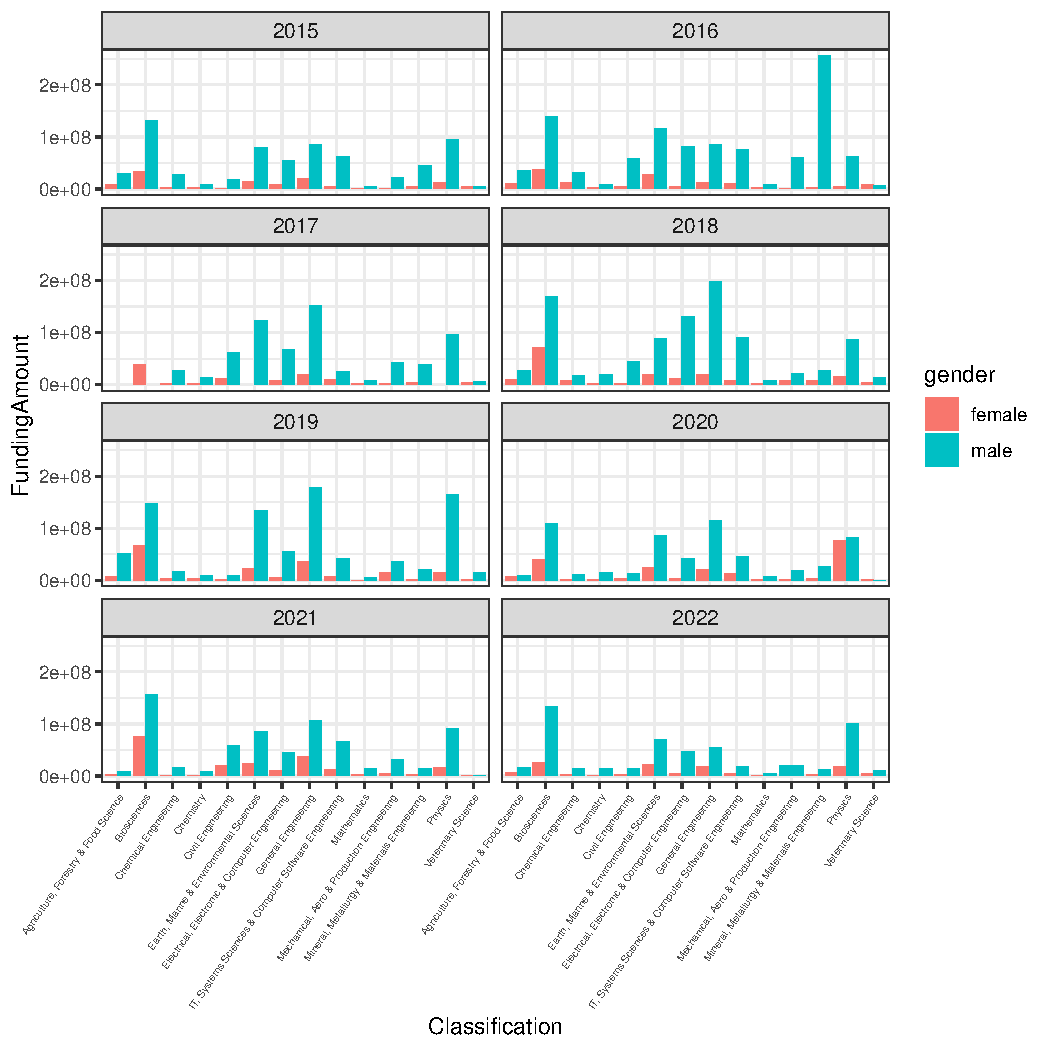
\includegraphics[width = 1\textwidth]{funding_all.pdf}
    \caption{The plot shows the total research funding allocated to each gender during the period measured in GBP.}
\end{figure}

From this result, a great gender gap is seen. The graph indicates that the gender gap in recent years is smaller compared to the first three years when the funding amount for females almost cannot be seen compared to males. The Biosciences field has the greatest amount of funding for females across time, except in 2020, when the gender gap in Physics is the smallest. Despite an emerging trend towards bridging the gender gap, the progress is subtle, and the overall scenario remains concerning.\\
\\
\noindent For the robustness of our result, a two-sample t-test is conducted for the number of funded males and females in different years. According to the result of the two-sample t-test, the t-statistic, representing the difference between the mean of the two data groups, is approximately 8.40; the p-value is 6.918e-14, much smaller than a significance level of 0.05. This result provides strong evidence to reject the null hypothesis, indicating a significant difference between the mean of research funding allocated to males and females from 2015 to 2022.

\subsection{Temporal trends comparison}

This subsection will display the comparison results for the temporal trends across the various STEM categories and institutions. The proportion of males and females getting funded will be shown in a time-series form. At the same time, I will show the ranking of the degree of bias across time to find the source of the disparity.

\subsubsection{Comparison among classifications}
\begin{figure}
    \centering
    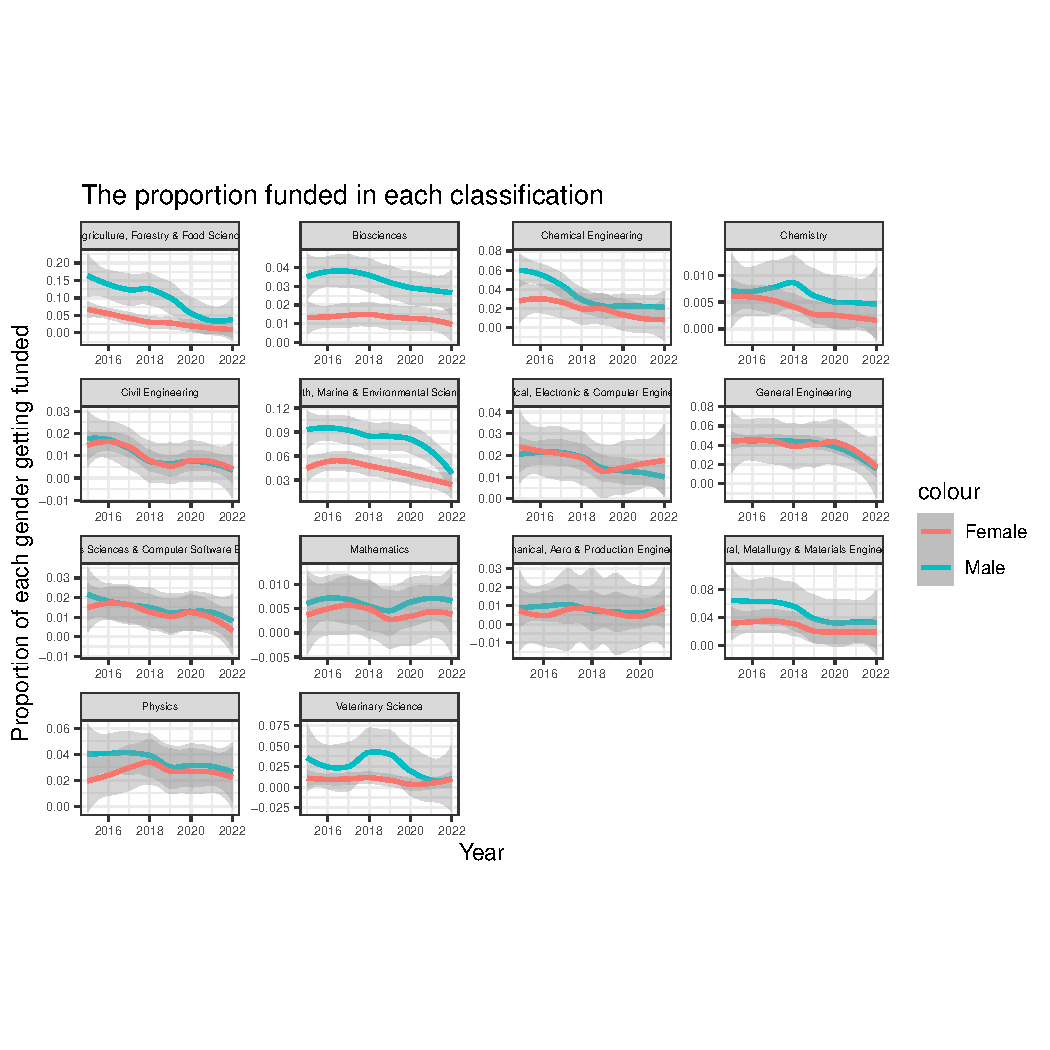
\includegraphics{plots_classification.pdf}
    \caption{This figure shows the general trend of funded proportion in each classification across time. In this result, the proportion of each gender is used, calculated by dividing the funded males or females by the total number of HESA staff in each gender. The grey area represents the 0.95 confidence interval - a narrower band usually indicates a more precise result.}
\end{figure}
\begin{figure}
	\centering
	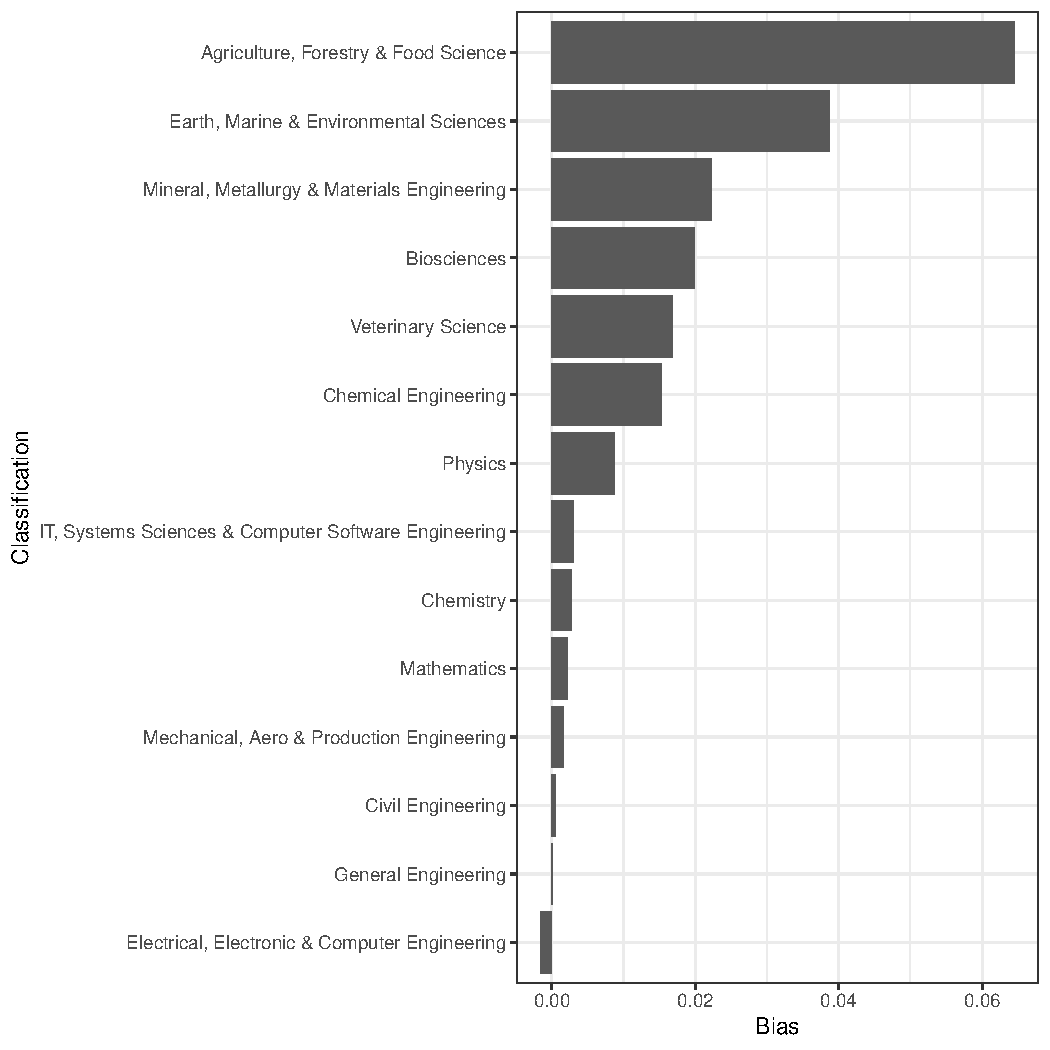
\includegraphics[width=0.8\textwidth]{rank_class.pdf}
	\caption{This figure shows the ranking of the extent of gender bias in each classification across time. For the bias degree, I calculated the total number of funded males or females from 2015 to 2022, divided by the total number of HESA staff in the corresponding gender during the period. Then, the difference of the ratios for males and females is conducted and is reordered depending on the degree of biases - the upper represents the classification with greater gender bias.}
\end{figure}

\noindent As displayed in Figures 2 and 3, the results show a great gender gap in the research funding of Biosciences, where the gap almost persists; though the extent of gender bias overall is the greatest in Agriculture, Forestry \& Food Science, the disparity has been considered diminished in the latest years. By contrast, there are several categories where the proportion of both genders is nearly the same over time, including General Engineering, Civil Engineering, and IT, Systems Sciences \& Computer Software Engineering. In most classifications, there is an encouraging trend indicating a reduction in the gap between males and females. An exception would be Chemistry, where the gender gap increased over time. An interesting observation is that in the field of Electrical, Electronic \& Computer Engineering, the proportion of funded females even exceeded that of males in recent years. 

\subsubsection{Comparison among universities}
As one of the primary criteria of the research application, university ranking would be an important factor that may affect funding fairness. The ratio of funded researchers in different universities is displayed in Figures 4 and 5, where each colour represents a classification, and the scales for each subplot were set to be the same; only the universities with sufficient funding data are selected for the comparison.
\begin{figure}
\caption{This figure shows the comparison among different universities. The results of 65 universities were generated in my study; however, only 12 of them were selected. The reason is that some of the universities have little funding data, therefore only the universities with the most number of results displayed are selected for analysis.}
\begin{tikzpicture}
    \node(img){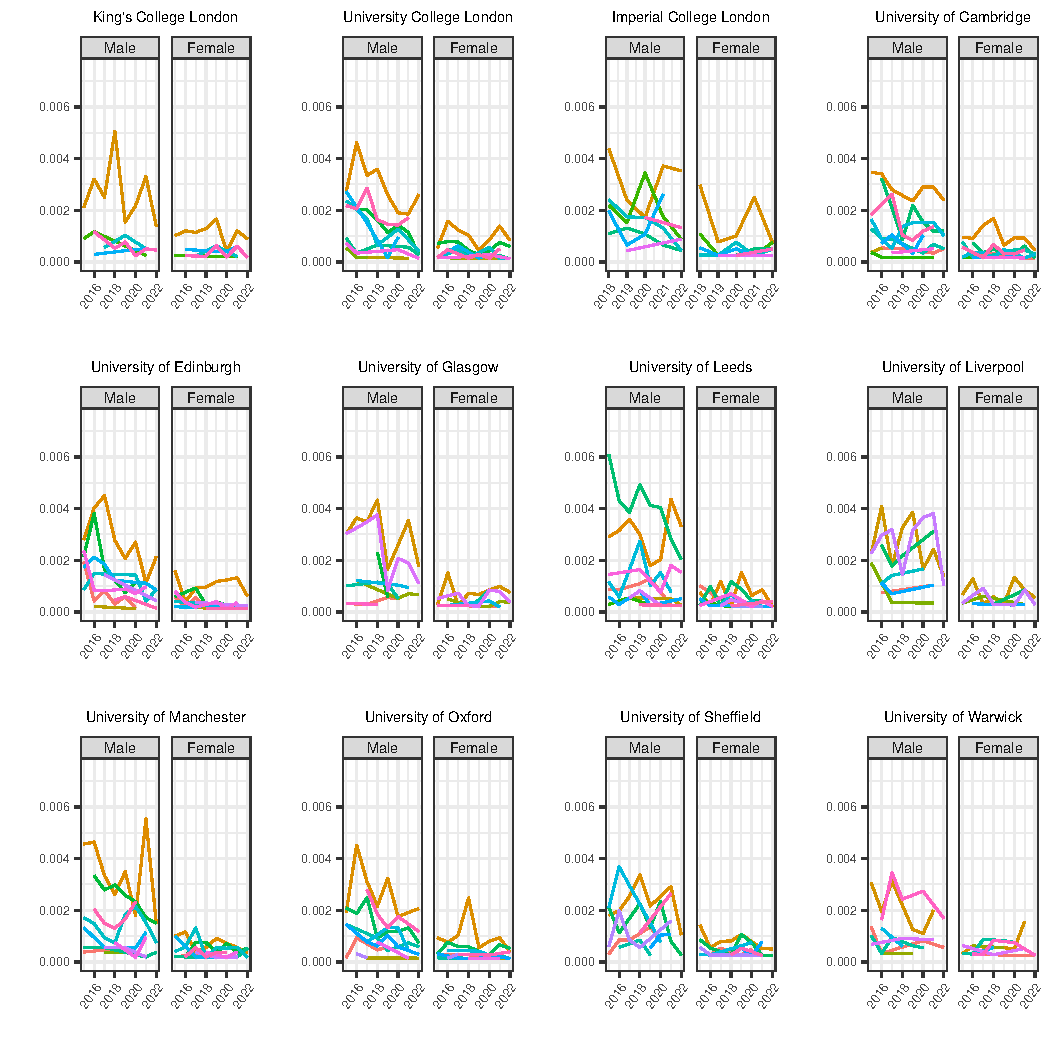
\includegraphics[page=1, scale=0.8]{uni_selected.pdf}};
    \node[below=of img, node distance=0cm, yshift=1cm,font=\color{black}\large] {Year};
    \node[left=of img, node distance=0cm, rotate=90, anchor=center,yshift=-0.7cm,font=\color{black}\large] {Ratio of each gender getting funded};
\end{tikzpicture}

\includegraphics[page=1, scale=0.6]{legend.pdf}
\end{figure}

\begin{figure}
	\centering
	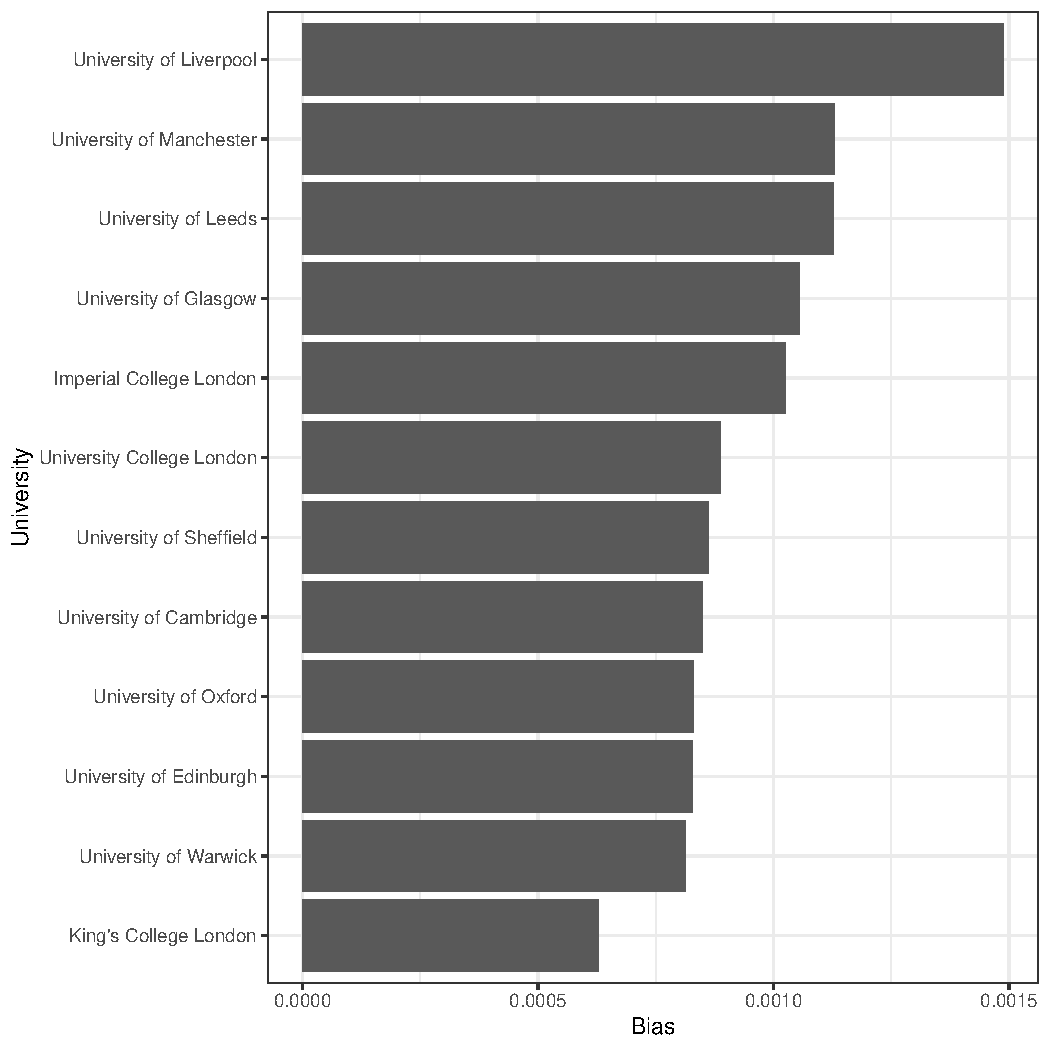
\includegraphics[height=0.7\textheight]{rank_uni.pdf}
	\caption{Similar to the previous comparison across various classifications, this figure shows the ranking of the extent of gender bias in universities. For each university, the total number of funded males or females in all classifications during the period 2015~2022 is summed up, and divided by the total number of HESA male or female staff in the corresponding university. The results are then used to calculate the degree of bias by finding the ratio for males minus the ratio for females in each university.}
\end{figure}

\noindent From the results shown, gender differences can be observed in all the universities we are studying. Among these universities, our results suggest that the gender gap at King's College London and the University of Warwick is comparatively smaller. In contrast, the gap in the other universities shows a baptism pattern with a larger gender gap. The gap is the largest for the results in the University of Liverpool and the University of Manchester compared to other institutions. We may conclude that the institution's ranking might potentially affect gender equality in STEM research funding. Additionally, a sad observation is that from this comparison result, there is no signal of an improving trend of reducing the gap. Though the ratio of funded males in recent years is decreasing, the reduction is also seen for females.

\pagebreak
\newpage
\section{Discussion}

The findings of this study point to a gender disparity in the overall pattern of research funding within the UK STEM sector, no matter the aspect of funding amount or funding ratio. A positive aspect is the partial reduction of this gap, which could be attributed to the growing focus on funding diversity. However, the beneficial impact is not evident and inequities persist. On the UKRI's official website, a commitment to gender equality is outlined, detailing the equality plan from 2022 to 2026. This plan encompasses transparency and monitoring of gender data, support for female leaders in the UK, efforts to address gender inequality in recruitment, etc. [\cite{plan}] However, to my knowledge, no actions in the plan specifically and directly address fair research funding between genders. Access to these resources remains unequal among different genders.\\
\\
This study also compared the trend across STEM categories over the years. The results showed several observations: 1) Despite the general trend of reducing the gender gap, the gap in Chemistry increased in recent years; 2) The gender gap in the funding ratio in Biosciences persists; 3) Though most engineering disciplines have a gender gap in funding amount, the gap in funding ratio is small; 4) The gap in Veterinary Science shows an opposite pattern, where females receive higher average amount of funding but lower funding ratio compared to males.

The findings indicate a decline in the gap across most categories, with the exception of Chemistry, where the disparities in both funding amount and funding ratio in recent years have grown compared to 2015. According to a 2018 report by the Royal Society of Chemistry, the relative percentage of female chemists advancing from undergraduate studies to senior academic roles has decreased by 35 percentage points [\cite{RoyalChemistry}]. The primary causes identified include arbitrary funding criteria and a lack of transparency in the recruitment and promotion process [\cite{RoyalChemistry}]. Despite efforts to reduce the gender gap [\cite{RSCFramework2023}], the gap only slightly decreased and continued beyond 2018. Biosciences exhibit a similar trend; the persistent funding ratio gap reveals no notable increase in the gender gap. Positively, there is no apparent gender disparity in the funding amount for funded researchers. It was noted that female researchers in biosciences are generally less successful in obtaining research funding. Previous research has shown that women with biological sciences degrees are less likely than men to work as scientists post-degree and tend to have shorter publishing careers, primarily due to leaving the field, and lower publishing rates as well [\cite{malespina2023gender}]. Contributing factors may include: 1. Gender disparities in the recruitment and promotion of women in biological sciences, similar to chemistry; 2. Differences in life goals between males and females may influence their decision-making [\cite{elliott2016editor}].\\

Another key result from my analyses is the gender disparity in funding amounts for engineering disciplines. Unlike the situation in Biosciences, the gender gap here is mainly observable in the amounts awarded, while gender equality in the funding ratio is relatively higher. This suggests that the funding structure could be a key factor in the gender imbalance in this sector. Based on information from the UKRI Engineering and Physical Sciences Research Council (EPSRC) \cite{UKRIengineering}, there are significant differences in the sizes of grants applied for by different genders, with female researchers consistently applying for smaller grants. Furthermore, the report points out that from 2007 to 2018, the award rates by value became increasingly different as the grant amounts increased \cite{UKRIengineering}. The award rate for women remained consistently around 30\% for all grant amounts, whereas for men it rose progressively from about 30\% to nearly 60\% as the grant amount increased. An EPSRC survey of female applicants revealed several reasons that might act as barriers to applying for larger grants \cite{UKRIsurvey}: 1. Lack of time due to being overwhelmed by other responsibilities; 2. Unfair biases in the peer review process; 3. Entry requirements for applications, such as institutional ranking or existing grant portfolio; 4. Absence of institutional support for large grant proposals. Notably, two of these primary causes are institution-related, which could indicate a troubling situation for female researchers. Previous research has shown that women are generally less likely to secure positions in highly ranked institutions compared to men \cite{gender_science}. Consequently, even though higher-ranked institutions may offer benefits to their female staff, the barriers to entering these institutions might prevent many women from accessing these advantages. This highlights potential inequities in resource allocation and possible biases in admission criteria.\\

The funding landscape in Veterinary Science reveals contrasting patterns: The average amount of funding for female researchers is generally higher than for male researchers, particularly in the first three years; however, male researchers have a higher funding ratio. This may be related to the significant representation of women in veterinary science, as evidenced by data from the Royal College of Veterinary Surgeons, which reported that in 2021, 77\% of practising veterinary surgeons in the UK were women [\cite{RCVS}]. Nevertheless, women are significantly underrepresented in journal publications - In 2023, 68\% of authors in a main journal of veterinary science, namely veterinary surgery, were men\cite{edinburgh_veterinary}]. The gendered masculine culture and the barriers mentioned in the previous paragraphs could be potential reasons for this phenomenon [\cite{liu2021women}]. In addition to the comparatively higher interest in this field by women, veterinary science is often considered a caring profession. Previous literature has proved the gendered nature in care professions, with women being more prevalent in part due to gender stereotypes such as men being less compassionate but more professional than women [\cite{poole1997caring}]. This also sheds light on why fewer women pursue academic careers in Veterinary Science, despite their high participation and graduation rates in veterinary programs, and why female academics are more likely to hold lower-ranked positions compared to their male colleagues [\cite{liu2021women}].
\\
\subsection{Implications and Recommendations}

In conclusion, our results revealed a significant gender bias in STEM research funding within the UK. Although there is a general decreasing trend for the gap, the academic framework continues to pose challenges to women. The internal link between research funding and the ranking of their institution could pose additional hurdles for female researchers. This could be regarded as a systematic bias in the review criteria, which benefits male applicants due to previous accumulative advantage [\cite{Holly2019}]. This inequality not only causes a reduction in the female researcher's incentive to deliver innovative studies that contribute to science, but would also be a factor influencing the career life of female researchers [\cite{jebsen2022dismantling}]. The number of research fundings, as an important role that affects the promotion of academic careers, would directly impact the retention and progression of female researchers [\cite{jebsen2022dismantling}], forming a vicious circle harmful to the situation of female researchers. To break the cycle, a systematic improvement in gender equality is necessary, which could include establishing a diversity focus group that monitors the diversity of the employment of each institution and ensures that the university recruitment process is fair and offers the same opportunity to various groups of people [\cite{sardelis2017ten}]. At the same time, this focus group should also be responsible for revising the funding application criteria, ensuring that the criteria could minimize the impact of accumulated advantage. 

\subsection{Limitations}
In this study, we conducted the trend comparison using the ratio of each gender getting funded, where the HESA staff data is used for the calculation. We assumed that the HESA staff number in each classification and university is the total number of researchers in these areas. In addition, another caveat that is worth noticing is that this study only considered females and males as the genders. All the other genders are not listed in consideration, while these are also worth more attention. Though this study mainly focuses on female researchers, it can be a broad indication of the situation of most minority groups [Jebsen et al. (2022)]. Lastly, the gender determination for each project is based on the name of the primary applicant, which could introduce some inaccuracy.\\
\\
\subsection{Future directions}

In this study, I have shown that there are gender biases among STEM disciplines, considering the total number of HESA staff to account for bias at all stages. However, to check the existing problem in the current diversity system, it would also be beneficial to study the funding trends based on the total number of applications so that we can find the proportion of bias caused during different stages, including the bias in the review stage and the step before application. In addition, this study only learned about the gender gap in STEM research funding. According to previous research, there may also be many other biases that may exist in research funding, including racial or nationality bias, ethnicity bias, risk aversion bias, etc. [\cite{wojick2015government}] All diversity should be as important as each other [\cite{LSE2018}], and bias in any aspect would have a direct impact on science innovation and career life of individuals. As such, more studies on other elements of discrimination should be conducted to increase awareness. 

\newpage
\section{Data and Code Availability}

In my study, the HESA staff data is sourced from the official HESA website, including staff number under various \href{https://www.hesa.ac.uk/data-and-analysis/staff/working-in-he/characteristics}{institutions} and \href{https://www.hesa.ac.uk/data-and-analysis/staff/areas#sex}{categories} over time. The project information from UKRI can be assessed from  \href{https://imperiallondon-my.sharepoint.com/personal/fcb5018_ic_ac_uk/_layouts/15/onedrive.aspx?id=\%2Fpersonal\%2Ffcb5018\%5Fic\%5Fac\%5Fuk\%2FDocuments\%2FFunding\%2DLandscape}{Onedrive}. The coding part is available on Github, including the \href{https://github.com/FCBT/Funding-Landscape}{machine-learning related part} and the \href{https://github.com/XW1722/Project}{analysis part}.
\newpage

\nocite{*}
\renewcommand{\bibname}{References}
\phantomsection
\addcontentsline{toc}{chapter}{References}
\bibliography{citation}
\end{document}